\documentclass{standalone}
\usepackage{tikz}
\usetikzlibrary{patterns, positioning}
\usepackage[sfdefault]{ClearSans} %% option 'sfdefault' activates Clear Sans as the default text font
\usepackage[T1]{fontenc}

\begin{document}
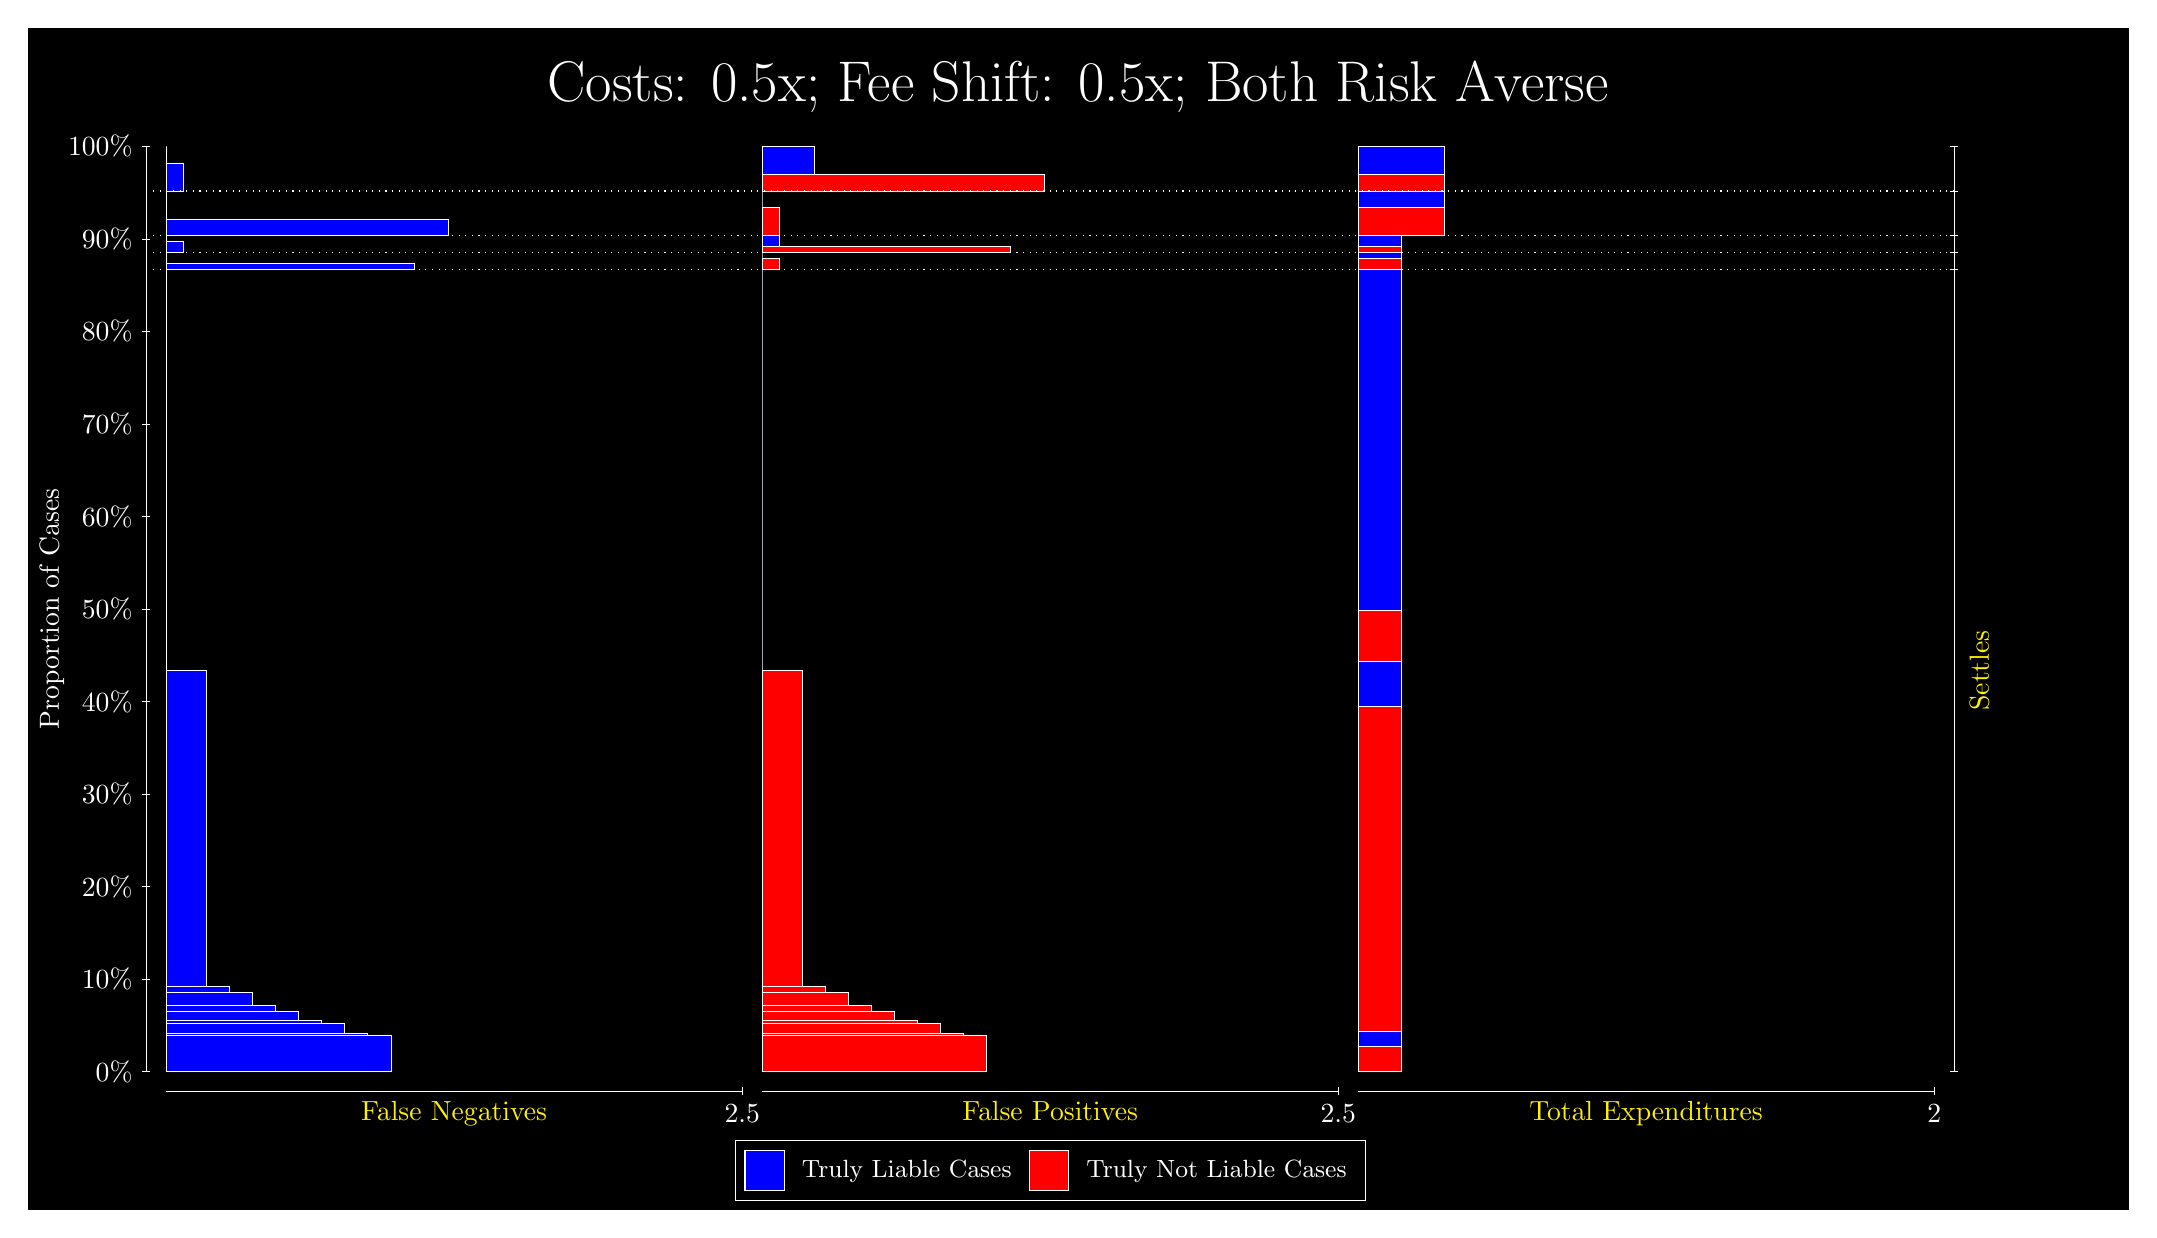
\begin{tikzpicture}
\draw[fill=black] (0,0) rectangle (26.667,15);
\draw[text=white] (0,13.5) rectangle (26.667,15) node[midway] {\huge Costs: 0.5x; Fee Shift: 0.5x; Both Risk Averse};
\draw[white, very thin] (1.5,1.75) -- (1.5,13.5);
\node[rotate=90, text=white, anchor=center] at (0.3, 7.625) {Proportion of Cases};
\draw[white, very thin] (1.45,1.75) -- (1.55,1.75);
\node[text=white, anchor=east] at (1.45, 1.75) {0\%};
\draw[white, very thin] (1.45,2.925) -- (1.55,2.925);
\node[text=white, anchor=east] at (1.45, 2.925) {10\%};
\draw[white, very thin] (1.45,4.1) -- (1.55,4.1);
\node[text=white, anchor=east] at (1.45, 4.1) {20\%};
\draw[white, very thin] (1.45,5.275) -- (1.55,5.275);
\node[text=white, anchor=east] at (1.45, 5.275) {30\%};
\draw[white, very thin] (1.45,6.45) -- (1.55,6.45);
\node[text=white, anchor=east] at (1.45, 6.45) {40\%};
\draw[white, very thin] (1.45,7.625) -- (1.55,7.625);
\node[text=white, anchor=east] at (1.45, 7.625) {50\%};
\draw[white, very thin] (1.45,8.8) -- (1.55,8.8);
\node[text=white, anchor=east] at (1.45, 8.8) {60\%};
\draw[white, very thin] (1.45,9.975) -- (1.55,9.975);
\node[text=white, anchor=east] at (1.45, 9.975) {70\%};
\draw[white, very thin] (1.45,11.15) -- (1.55,11.15);
\node[text=white, anchor=east] at (1.45, 11.15) {80\%};
\draw[white, very thin] (1.45,12.325) -- (1.55,12.325);
\node[text=white, anchor=east] at (1.45, 12.325) {90\%};
\draw[white, very thin] (1.45,13.5) -- (1.55,13.5);
\node[text=white, anchor=east] at (1.45, 13.5) {100\%};

\draw[white, very thin] (24.457,1.75) -- (24.457,13.5);
\draw[white, very thin] (24.407,1.75) -- (24.507,1.75);
\node[anchor=west] at (24.407, 1.75) {};
\draw[white, very thin] (24.407,11.937) -- (24.507,11.937);
\node[anchor=west] at (24.407, 11.937) {};
\draw[white, very thin] (24.407,12.151) -- (24.507,12.151);
\node[anchor=west] at (24.407, 12.151) {};
\draw[white, very thin] (24.407,12.365) -- (24.507,12.365);
\node[anchor=west] at (24.407, 12.365) {};
\draw[white, very thin] (24.407,12.933) -- (24.507,12.933);
\node[anchor=west] at (24.407, 12.933) {};
\draw[white, very thin] (24.407,13.5) -- (24.507,13.5);
\node[anchor=west] at (24.407, 13.5) {};

\draw[white, very thin, fill=blue] (1.75,1.75) rectangle (4.6044,2.2065);
\draw[white, very thin, fill=blue] (1.75,2.2065) rectangle (4.3116,2.2396);
\draw[white, very thin, fill=blue] (1.75,2.2396) rectangle (4.0188,2.3638);
\draw[white, very thin, fill=blue] (1.75,2.3638) rectangle (3.7261,2.397);
\draw[white, very thin, fill=blue] (1.75,2.397) rectangle (3.4333,2.5154);
\draw[white, very thin, fill=blue] (1.75,2.5154) rectangle (3.1406,2.5905);
\draw[white, very thin, fill=blue] (1.75,2.5905) rectangle (2.8478,2.7567);
\draw[white, very thin, fill=blue] (1.75,2.7567) rectangle (2.5551,2.8318);
\draw[white, very thin, fill=blue] (1.75,2.8318) rectangle (2.2623,6.8436);
\draw[white, very thin, fill=red] (1.75,6.8436) rectangle (1.75,11.937);
\draw[white, very thin, fill=blue] (1.75,11.937) rectangle (4.8971,12.013);
\draw[white, very thin, fill=red] (1.75,12.013) rectangle (1.75,12.151);
\draw[white, very thin, fill=blue] (1.75,12.151) rectangle (1.9696,12.29);
\draw[white, very thin, fill=red] (1.75,12.29) rectangle (1.75,12.365);
\draw[white, very thin, fill=blue] (1.75,12.365) rectangle (5.3362,12.577);
\draw[white, very thin, fill=red] (1.75,12.577) rectangle (1.75,12.933);
\draw[white, very thin, fill=blue] (1.75,12.933) rectangle (1.9696,13.289);
\draw[white, very thin, fill=red] (1.75,13.289) rectangle (1.75,13.5);
\draw[white, very thin, fill=red] (9.3189,1.75) rectangle (12.173,2.2065);
\draw[white, very thin, fill=red] (9.3189,2.2065) rectangle (11.88,2.2396);
\draw[white, very thin, fill=red] (9.3189,2.2396) rectangle (11.588,2.3639);
\draw[white, very thin, fill=red] (9.3189,2.3639) rectangle (11.295,2.397);
\draw[white, very thin, fill=red] (9.3189,2.397) rectangle (11.002,2.5154);
\draw[white, very thin, fill=red] (9.3189,2.5154) rectangle (10.709,2.5905);
\draw[white, very thin, fill=red] (9.3189,2.5905) rectangle (10.417,2.7567);
\draw[white, very thin, fill=red] (9.3189,2.7567) rectangle (10.124,2.8318);
\draw[white, very thin, fill=red] (9.3189,2.8318) rectangle (9.8312,6.8435);
\draw[white, very thin, fill=blue] (9.3189,6.8435) rectangle (9.3189,11.937);
\draw[white, very thin, fill=red] (9.3189,11.937) rectangle (9.5384,12.076);
\draw[white, very thin, fill=blue] (9.3189,12.076) rectangle (9.3189,12.151);
\draw[white, very thin, fill=red] (9.3189,12.151) rectangle (12.466,12.227);
\draw[white, very thin, fill=blue] (9.3189,12.227) rectangle (9.5384,12.365);
\draw[white, very thin, fill=red] (9.3189,12.365) rectangle (9.5384,12.722);
\draw[white, very thin, fill=blue] (9.3189,12.722) rectangle (9.3189,12.933);
\draw[white, very thin, fill=red] (9.3189,12.933) rectangle (12.905,13.144);
\draw[white, very thin, fill=blue] (9.3189,13.144) rectangle (9.9776,13.5);
\draw[white, very thin, fill=red] (16.888,1.75) rectangle (17.437,2.0664);
\draw[white, very thin, fill=blue] (16.888,2.0664) rectangle (17.437,2.2568);
\draw[white, very thin, fill=red] (16.888,2.2568) rectangle (17.437,6.387);
\draw[white, very thin, fill=blue] (16.888,6.387) rectangle (17.437,6.9619);
\draw[white, very thin, fill=red] (16.888,6.9619) rectangle (17.437,7.6089);
\draw[white, very thin, fill=blue] (16.888,7.6089) rectangle (17.437,11.937);
\draw[white, very thin, fill=red] (16.888,11.937) rectangle (17.437,12.076);
\draw[white, very thin, fill=blue] (16.888,12.076) rectangle (17.437,12.151);
\draw[white, very thin, fill=red] (16.888,12.151) rectangle (17.437,12.227);
\draw[white, very thin, fill=blue] (16.888,12.227) rectangle (17.437,12.365);
\draw[white, very thin, fill=red] (16.888,12.365) rectangle (17.986,12.722);
\draw[white, very thin, fill=blue] (16.888,12.722) rectangle (17.986,12.933);
\draw[white, very thin, fill=red] (16.888,12.933) rectangle (17.986,13.144);
\draw[white, very thin, fill=blue] (16.888,13.144) rectangle (17.986,13.5);
\draw[white, dotted] (1.5,11.937) -- (24.457,11.937);
\draw[white, dotted] (1.5,12.151) -- (24.457,12.151);
\draw[white, dotted] (1.5,12.365) -- (24.457,12.365);
\draw[white, dotted] (1.5,12.933) -- (24.457,12.933);
\draw[white, very thin] (1.75,1.5) -- (9.0689,1.5);
\node[text=yellow, anchor=north] at (5.4094, 1.5) {False Negatives};
\draw[white, very thin] (9.0689,1.45) -- (9.0689,1.55);
\node[text=white, anchor=north] at (9.0689, 1.45) {2.5};

\draw[white, very thin] (9.3189,1.5) -- (16.638,1.5);
\node[text=yellow, anchor=north] at (12.978, 1.5) {False Positives};
\draw[white, very thin] (16.638,1.45) -- (16.638,1.55);
\node[text=white, anchor=north] at (16.638, 1.45) {2.5};

\draw[white, very thin] (16.888,1.5) -- (24.207,1.5);
\node[text=yellow, anchor=north] at (20.547, 1.5) {Total Expenditures};
\draw[white, very thin] (24.207,1.45) -- (24.207,1.55);
\node[text=white, anchor=north] at (24.207, 1.45) {2};

\node[text=yellow, centered, rotate=90] at (24.777, 6.8436) {Settles};





\draw (12.978300999999998,1.5) node[draw=none] (baseCoordinate) {};
\begin{scope}[align=center]
        \matrix[scale=0.5, draw=white, below=0.5cm of baseCoordinate, nodes={draw}, column sep=0.1cm]{
            \node[rectangle, draw, minimum width=0.5cm, minimum height=0.5cm, fill=blue] {}; &
            \node[draw=none, font=\small, text=white] (B) {Truly Liable Cases}; &
            \node[rectangle, draw, minimum width=0.5cm, minimum height=0.5cm, fill=red] {}; &
            \node[draw=none, font=\small, text=white] (B) {Truly Not Liable Cases}; \\
            };
\end{scope}

\end{tikzpicture}
\end{document}